\documentclass{beamer}
\usetheme{manhattan}  % Now it's a beamer presentation with the Manhattan College theme!

\usepackage{url}

% Make a new command that will make a new subsection and a frame with the same title
\newcommand{\fst}[2]{\subsection{#1}\frame{\frametitle{#1} #2}}

\title{Drawing Trees and Animating Tree Changes}
\author[Badame and Boothe]{Sandro Badame \and Peter Boothe*}
\date{9 March 2010}
\institute[Manhattan College]{
    \url{{sbadame.student,peter.boothe}@manhattan.edu}\\
    Mathematics and Computer Science \\
    Manhattan College}

\begin{document}
\frame{\titlepage}

\section{Introduction}

\fst{The Problem}{
\begin{itemize}
\item Trees undergoing changes occur in many contexts
    \begin{itemize}
        \item Visualization can be a help 
    \end{itemize}
\item Writing graphics and layout code from the ground up is hard.
\item Writing animation code is harder
\item Worst of all often the people who have skills with algorithms have little 
  experience with graphics programming.
    \begin{itemize}
        \item And vice-versa
    \end{itemize}
\end{itemize}
}

\fst{Our Solution}{
\begin{itemize}
\item We have built a Java library for displaying trees and animating tree changes
\item To demonstrate the generality of the library we have created three example visualizations.
    \begin{enumerate}
        \item AVL Trees
        \item Tree Automata
        \item LISP/Scheme
    \end{enumerate}
\end{itemize}
}

\fst{How It Works}{
    \centering
    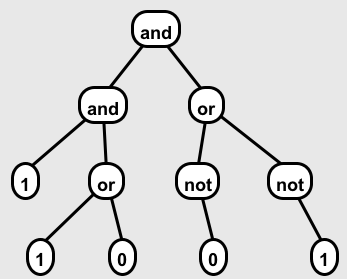
\includegraphics[width=1.75in]{example.png}

    \begin{itemize} 
        \item Each vertex is a magnet that repulses its neighbors
        \item Each edge is a spring, pulling adjacent vertices closer
        \item Each vertex has a fixed vertical position and a fixed horizontal order
        \item As the tree changes, the physical system adjusts
    \end{itemize} 
}

\section{Demonstrations}

\fst{AVL Trees}{
\begin{itemize}
    \item Example of self-adjusting binary search trees
    \item AVL Tree invariant: The left and right subtree of a node differ in maximum depth by no more than 1
    \item If this invariant is violated, fix the tree via rotations
\end{itemize}
}

\fst{Tree Automata}{
\begin{itemize}
    \item Take as input trees rather than strings.
    \item Progressively rewrite the input tree until either
    \begin{itemize}
        \item There is no rule to transform the tree (reject) \\
            ~~~~OR
        \item The tree is isomorphic to a member of the set of base trees  (accept)
    \end{itemize}
\end{itemize}
}

\frame{
\frametitle{Our Tree Automaton: Tautology Checker}
    \begin{description}
        \item{\bf Base Trees:} $$\{ q1 \}$$

        \item{\bf Rewrite Rules:}

~\\

    \hspace{-.8in}
      \begin{tabular}{c | c | c}
         $1 \to q1$         & $(AND ~q1 ~q0) \to q0$ & $(OR ~q1 ~q0) \to q1$ \\
         $0 \to q0$         & $(AND ~q1 ~q1) \to q1$ & $(OR ~q1 ~q1) \to q1$ \\
         $(NOT ~q1) \to q0$ & $(AND ~q0 ~q0) \to q0$ & $(OR ~q0 ~q0) \to q0$ \\
         $(NOT ~q0) \to q1$ & $(AND ~q0 ~q1) \to q0$ & $(OR ~q0 ~q1) \to q1$ 
        \end{tabular}
    \end{description}
}
  
\fst{Scheme/Lisp}{
    \begin{itemize} 
        \item Scheme/Lisp code represents the Abstract Syntax Tree directly.
        \item Executing Scheme code corresponds to manipulation of the AST

           $\therefore$ We can animate the execution of Scheme code
    \end{itemize}
}
        
\frame{
    \frametitle{Summary of Examples}
    \begin{itemize} 
        \item These animations were not too hard to write.
        \item The extra code required to perform the animation was on the order of 10 lines of Java code. 
        \item The same library is used for all animations.
        \item We feel that we have created a library that can be useful in a wide variety of situations.
    \end{itemize} 
}

\section{Wrapping Up}

\fst{Conclusion}{
    \begin{itemize} 
        \item Write visualizations for yourself 
        \item Get your students to write them
        \item \url{http://github.com/pboothe/Lispy-Animator}
        \item Any Questions?
    \end{itemize} 
}

\end{document}
